
\begin{frame}
  \frametitle{Context}
  \begin{itemize}
  \item 2 types of models for CECSP/RCPSP: Time-indexed and Event-based
    \vfill
    \pause
  \item TI model more efficient {\small (relatively stronger relaxation)}
    \pause
    \vfill
  \item But:
    \begin{itemize}
    \item  model size depends on planning horizon 
      
      {\footnotesize  $\longrightarrow $ for large planning horizon event-based model can be more
        efficient (RCPSP:~{\color{gray!50!black!70}\it [Koné et al.,
          2011]} )}
      \vfill
      \pause
    \item only integer solutions
      
      {\footnotesize $\longrightarrow$ time-indexed model can lead to
        infeasible/sub-optimal solution
        (CECSP:~{\color{gray!50!black!70}\it [Nattaf et al., 2015]} )}
    \end{itemize}
  \end{itemize}
  \vfill
  \pause
  {\bf Goal: Tightened Event-based models (2 formulations)} 
\end{frame}

\subsection{Event-based formulations}
\begin{frame}{Event-based model}
  \vfill
  \begin{itemize}
  \item 2 event based model : Start/End and On/Off
    \vfill
    \pause
  \item Start/End model have stronger relaxations than the On/Off
    model ( $\mathbf{var(OO) = func\, (var (SE))}$)
    \pause
    \vfill
  \item But: On/Off model has less variables than Start/End model
    \pause
    and  better performances  
    \vfill
    \pause
  \item Study of the On/Off formulation
    \vfill
    \pause
  \item Improvement of the formulation: collaboration with Tam{\'a}s Kis 
  \end{itemize} 
  \vfill
\end{frame}

\begin{frame}
  \frametitle{On/Off formulation}
  {\small \it Adaptation of a model for the RCPSP {\color{gray!50!black!50} \it [Koné et al., 2011]}}
  \vfill
  \pause
  \begin{block}{Variables}
    \begin{itemize}
    \item  $t_e$ represents the event (start or end time)
      \pause
      \vspace{0.3cm}
    \item $z_{ie}=\left\{
        \begin{array}{ll}
          1 & \text{if $i$ is in process during $[t_{e},t_{e+1}]$}\\
          0 & \text{sinon}
        \end{array}
      \right.
      $
      \pause
      \vspace{0.3cm}
    \item $B_{ie}$: resource quantity consumed by $i$ in $\inter[t_e][t_{e+1}]$
      \vspace{0.3cm}
    \item $W_{ie}$: energy brought to $i$ in $\inter[t_e][t_{e+1}]$   
    \end{itemize}
  \end{block}
\end{frame}







\subsection{Valid inequalities}
\begin{frame}
  \frametitle{Maximum separation between events}
  % \begin{itemize}
  % \item {\bf Goal: } upper bound on the value of $t_{e+1}-t_{e}$
  %   \vspace{0.3cm}
  % \item<2-> Time window of each task start and/or end time
  %   \vspace{0.3cm}
  % \item<6-> An event must occur in each of these time windows
  %   \vspace{0.3cm}
  % \item<11-> two consecutive events in the union of two consecutive time windows
  % \end{itemize}
  \begin{itemize}
  \item {\bf Goal: } upper bound on the value of $t_{e+1}-t_{e}$
    \vfill
  \item Consider the following example with 2 tasks:  
    \vfill
    \begin{center} 
      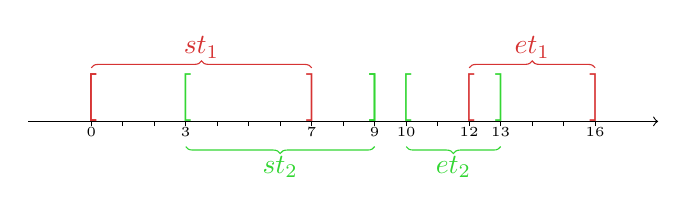
\begin{tikzpicture}
        [decoration={brace},scale=0.4]
        \node (O) at (0,0) {}; 
        \draw[->] (-2,0) -- (18,0);

        \foreach \i in {0,...,16}{
          \draw (\i,-0.15) -- (\i,0);
        }
        \onslide<1-2,4>{  \path (0,0) node[color=red!80!black!80,above=-0.12cm] {\LARGE [} --
          +(0:7cm)node[color=red!80!black!80,above=-0.12cm] {\LARGE ]};}
        \onslide<1,3-4>{\path[green!80!black!80](3,0) node[above=-0.12cm] {\LARGE [} -- +(0:6cm)
          node[above=-0.12cm]  {\LARGE ]};}
        \onslide<1>{ \path[green!80!black!80] (10,0) node[above=-0.12cm]  {\LARGE [}  --
          +(0:3cm) node[above=-0.12cm]  {\LARGE ]}  ;
          \path (12,0) node[color=red!80!black!80,above=-0.12cm] {\LARGE [} --
          +(0:4cm) node[color=red!80!black!80,above=-0.12cm] {\LARGE ]} ; }
        
        \path (0,0) node[below=-0.05cm] {\tiny 0} --
        +(0:7cm) node[below=-0.05cm]{\tiny 7};
        \path (3,0) node[below=-0.05cm]{\tiny 3} -- +(0:6cm)
        node[below=-0.05cm]{\tiny 9};
        \path (10,0) node[below=-0.05cm]{\tiny 10}  --
        +(0:3cm) node[below=-0.05cm]{\tiny 13}  ;
        \path (12,0) node[below=-0.05cm]{\tiny 12} --
        +(0:4cm) node[below=-0.05cm]{\tiny 16} ; 
        

        \onslide<1-2,4>{\draw [decorate,color=red!80!black!80] (0,1.7) -- +(0:7cm)
          node[midway,above]{$st_1$}; }
        \onslide<1>{ \draw [decorate,color=red!80!black!80] (12,1.7) -- +(0:4cm)
          node[midway,above] {$et_1$};}

        \onslide<1,3-4>{ \draw [decorate,green!80!black!80] (9,-0.8) -- +(0:-6cm)
          node[midway,below] {$st_2$};}
        \onslide<1>{   \draw [decorate,green!80!black!80] (13,-0.8) -- +(0:-3cm)
          node[midway,below] {$et_2$};}  
        \onslide<4->{  \draw (0,0)
          node[color=red!80!black!80,above=-0.12cm] {\LARGE [} ;
          \draw[green!80!black!80](9,0) node[above=-0.12cm] {\LARGE ]} ;}
        
      \end{tikzpicture}
    \end{center}
    {\color{gray!60!black!70} \small $2$ tasks $\Rightarrow 4$ events:
      $t_1,\ t_2,\ t_3$ and $t_4$}
  \item<2-> $t_1 \in [0,7]$ \onslide<3->{and $t_2 \in [3,9]$}
    \vfill
  \item<4-> What deduction about $t_2 - t_1$ ?
    
    $t_1,t_2 \in [0,9] \Rightarrow \mathbf{t_2-t_1 \le 9}$
    
  \end{itemize}
  
\end{frame}


\begin{frame}{Maximum separation between events}
  \vfill
  \begin{itemize}
  \item Can be generalized to any pair of events
    \vfill
  \item Can be used as:
    \begin{itemize}
      \vspace{0.2cm}
    \item additional constraints of the model
    \item instead of $M$ in min consump. constraint
    \end{itemize}  
    \vfill
  \item Same reasoning can be used to deduce bound on $t_e$

    {\small \color{gray!60!black!70} {\bf Idea} consider upper bound
      of $[est-i,lst_i]/[eet_i,let_i]$ instead of the whole interval}
    \vfill
  \end{itemize}
\end{frame}


% \begin{frame}
%   \frametitle{Maximum separation between events}
%   \begin{itemize}
%   \item Order the time-window intervals according to:
%     \[ [a,b] \le [c,d]
%       \Leftrightarrow a < c \lor \left( a=c \land b \le d\right)\]
%     \vfill
%     \pause
%   \item Then we have:
%     \[t_{e+1}-t_e  \le   |tw_e \cup tw_{e+1}|    \]
%     \pause
%     \begin{flushright}
%       \textcolor{black!70}{\scriptsize in fact: $t_{e+1}-t_e  \le
%       \overline{tw_e \cup tw_{e+1}} - \underline{tw_e \cup tw_{e+1}}
%       $}
%     \end{flushright}
%     \pause
%     \vfill
%   \item We can use it as:
%     \begin{itemize}
%       \vspace{0.2cm}
%     \item additional constraints of the model
%     \item an upper bound on $t_{e+1}-t_e$ in any constraints using a worst one
%     \end{itemize}
%   \end{itemize}
% \end{frame} 

% \begin{frame}
%   \frametitle{Maximum time for an event}
%   \begin{itemize}
%   \item {\bf Goal: } upper bound on the value of $t_{e}$
%     \vspace{0.4cm}
%   \item<2-> upper bound of each task start and/or end time
%     \vspace{0.4cm}
%   \item<5-> an event must occur before each of these upper bounds
%     \vspace{0.4cm}
%   \end{itemize}
%   \vfill
%   \onslide<3->{
%   \begin{center} 
%     \begin{tikzpicture}
%       [decoration={brace},scale=0.4]
%       \node (O) at (0,0) {}; 

%       \draw[->] (0,0) -- (19,0);
%       \onslide<3>{
%       \draw (1,0) node {\LARGE [} -- +(0:5cm)node {\LARGE ]}; 

%       \draw(4,0) node {\LARGE [} -- +(0:4cm) node {\LARGE ]} ;

%       \draw (8.05,0) node {\LARGE [}  --
%       +(0:6cm) node {\LARGE ]}  ;
%       \draw (12,0) node {\LARGE [} --
%       +(0:6cm) node {\LARGE ]}  ;}
%       \onslide<4>{

%       \draw (1,0) node {} -- +(0:5cm)node {\LARGE ]}; 

%       \draw(4,0) node {} -- +(0:4cm) node {\LARGE ]} ;

%       \draw (8.05,0) node {}  --
%       +(0:6cm) node {\LARGE ]}  ;
%       \draw (12,0) node {} --
%       +(0:6cm) node {\LARGE ]}  ;}
%       \onslide<5>{
%       \draw[color=blue!80!black!50] (0,0) node {} -- +(0:6cm)node {\LARGE ]}
%       node[left,above=0.8cm] {$t_0$}; 
%       \draw (8,0) node {\LARGE ]} ;
%       \draw (8.05,0) node {}  -- +(0:6cm) node {\LARGE ]}  ;
%       \draw (12,0) node {} -- +(0:6cm) node {\LARGE ]}  ;}

%       \onslide<6>{
%       \draw (6,0) node  {\LARGE ]}; 
%       \draw[color=blue!80!black!50](0,0) -- (8,0) node {\LARGE ]} node[left,above=0.8cm] {$t_1$};
%       \draw (8.05,0) node {}  --  +(0:6cm) node {\LARGE ]}  ;
%       \draw (12,0) node {} --  +(0:6cm) node {\LARGE ]}  ;}

%       \onslide<7>{
%       \draw (6,0) node {\LARGE ]}; 
%       \draw (8,0) node {\LARGE ]} ;
%       \draw[color=blue!80!black!50] (0,0) node {}  -- (14,0) node {\LARGE ]} node[left,above=0.8cm] {$t_2$} ;
%       \draw (18,0)node {\LARGE ]}  ;}

%       \onslide<8>{
%       \draw (6,0) node {\LARGE ]}; 
%       \draw(8,0) node {\LARGE ]} ;
%       \draw (14,0) node {\LARGE ]}  ;
%       \draw[color=blue!80!black!50] (0,0) node {} -- (18,0) node {\LARGE ]}
%       node[left,above=0.8cm] {$t_3$};} 

%     \end{tikzpicture}
%   \end{center}
% }
% \end{frame}


% \begin{frame}
%   \frametitle{Maximum time for an event}
%   \begin{itemize}
%   \item Order the time-window interval upper bounds ${\cal UP}$ in
%     increasing order 
%     \vfill
%     \pause
%   \item Then we have:
%     \[t_e \le  {\cal UP}_e\]
%     \vfill
%     \pause
%   \item We can use it as:
%     \begin{itemize}
%       \vspace{0.2cm}
%     \item additional constraints of the model
%     \item an upper bound on $t_{e+1}-t_e$ in any constraints using a worst one
%     \end{itemize}
%   \end{itemize}
% \end{frame}

\subsection{Polyhedral results}


\begin{frame}
  \frametitle{$Z_i$-polyhedron}
  \vspace{0.5cm}
  \onslide<1->{$\rightarrow$ Minimal set of inequalities defining the
    {\it ``$Z_i$-polyhedron''}.}
  \vspace{0.6cm}
  \onslide<2-> {  \begin{block}{$Z_i$-polyhedron}
      form of $z_i \in \{0,1\}^{|{\cal E}|}$ solution? \hspace{2.5cm}
      {\scriptsize (${\cal E}=$event set)}}
    \vspace{0.4cm}

    \onslide<4->{$\Rightarrow$ vector with consecutive-one property  and at least
      one $1$
      \begin{center}
        {\small e.g. $(0,0,1,1,1,0),\ (1,1,1,0,0,0),\ \dots$}
      \end{center}}
    \onslide<5->{     
      \[Z_i= conv\{z_i \in \{0,1\}^{|{\cal E}|} | z_i \text{ of the
          form } (0^*\, 1\, 1^*\, 0^*)\} \] }
    \vspace{-0.2cm}
  \end{block}
  \onslide<3->{\textcolor{black!70}{ \small\[z_{ie}=\left\{
          \begin{array}{ll}
            1 & \text{if task $i$ is in process between $t_e$ and $t_{e+1}$}\\
            0 & \text{otherwise}
          \end{array}
        \right.
      \]}}
\end{frame}


\begin{frame}
  \frametitle{Computational experience}
  \begin{itemize}
    \vfill
  \item Intel Core i7-4770 processor with 4 cores and 8Go of RAM
    \vfill
  \item OS: 64-bit Ubuntu 12.04
    \vfill
  \item MILP resolution: CPLEX 12.6 with 1 thread  
    \vfill
  \item Special separation procedure for non-preemptive cuts ($O(n^2)$)
    for node with depth less than 10 (Preem.)
    \vfill
  \item time limit: 1000 seconds
    \vfill
  \end{itemize}
\end{frame}

\pgfplotstableread[row sep=\\,col sep=&]{
  tasks & Default & Int. & Time & Preem. & I+T+P \\
  20    & 164.14 & 182.2 & 167.3 & 330.9 & 154  \\
  25     & 635.4 & 727.3 & 629.5 & 822.4 & 389.9 \\
  30    & 968  & 851 & 961.4 & 914.8 & 813.8\\
}\mydata

\begin{frame}
  \frametitle{Time comparison for the CECSP}
  \begin{itemize}
  \item Instances of {\it [Nattaf et al.,2015]}
  \item 10 instances of 20, 25 and 30 tasks
  \end{itemize}

  \vspace{0.2cm}
  \begin{center}\begin{tikzpicture}
      \begin{axis}[ enlarge x limits=0.25,
        ybar,
        bar width=.4cm,  
        legend style={at={(0.5,1)},
          anchor=north,legend columns=-1},
        width=\textwidth,
        height=.6\textwidth,
        symbolic x coords={20,25,30},
        xtick=data,
        ymin=0,ymax=1100,
        ylabel={\small time (s)},
        xlabel={\small $\#tasks$}]
        \addplot table[x=tasks,y=Default]{\mydata};
        \addplot table[x=tasks,y=Int.]{\mydata};
        \addplot table[x=tasks,y=Time]{\mydata};
        \addplot table[x=tasks,y=Preem.]{\mydata};
        \addplot table[x=tasks,y=I+T+P]{\mydata};
        \legend{Default, $t_{e+1}-t_e$ , $t_e$ , Preem. , three}
      \end{axis}
    \end{tikzpicture}
  \end{center}
\end{frame}

\pgfplotstableread[row sep=\\,col sep=&]{
  tasks & Default & Int. & Time & Preem. & I+T+P \\
  20    & 90.9 & 90.9 & 90.9 & 72.7 & 90.9\\
  25     &55.6 & 55.6 & 88.9 & 44.4 & 77.8\\
  30    & 10 & 20& 20& 10 &60\\
}\mydat
\begin{frame}
  \frametitle{Solved instances comparison for the CECSP}
  \begin{itemize}
  \item Instances of {\color{gray!50!black!70}\it [Nattaf et al., 2015]}
  \item 10 instances of 20, 25 and 30 tasks
  \end{itemize}

  \vspace{0.2cm}
  \begin{center}\begin{tikzpicture}
      \begin{axis}[ enlarge x limits=0.25,
        ybar,
        bar width=.4cm,  
        legend style={at={(0.5,1)},
          anchor=north,legend columns=-1},
        width=\textwidth,
        height=.6\textwidth,
        symbolic x coords={20,25,30},
        xtick=data,
        ymin=0,ymax=110,
        ylabel={\small $\%solved$},
        xlabel={\small $\#tasks$}]
        \addplot table[x=tasks,y=Default]{\mydat};
        \addplot table[x=tasks,y=Int.]{\mydat};
        \addplot table[x=tasks,y=Time]{\mydat};
        \addplot table[x=tasks,y=Preem.]{\mydat};
        \addplot table[x=tasks,y=I+T+P]{\mydat};
        \legend{Default, $t_{e+1}-t_e$ , $t_e$ , Preem. , three}
      \end{axis}
    \end{tikzpicture}
  \end{center}
\end{frame}

